\mychapter{MCTest+Moodle+VPL}\label{ch:experimentos_VPL}

Neste capítulo, serão apresentados resumos dos artigos que relatam os métodos e experimentos de integração entre o MCTest e o Moodle, com foco especial na utilização do \textit{plugin} VPL. A maioria desses artigos já foi detalhada em capítulos anteriores deste livro e, portanto, não será refeita a apresentação completa. Os experimentos foram realizados principalmente nas disciplinas de Bases Computacionais da Ciência (CS0) e Processamento da Informação (CS1) do Bacharelado em Ciência e Tecnologia da Universidade Federal do ABC (UFABC).

\section{MCTest-5, com Moodle}

%%%%%%%%%%%%%%%%%%%%%%%%%%%%%%%%%%%%%%%%%%%%%%%%%%%%%%%%%%%%%%%%%%%%%%%%%
\subsection*{Artigo sobre a exportação de questões paramétricas para o Moodle usando o MCTest}
%%%%%%%%%%%%%%%%%%%%%%%%%%%%%%%%%%%%%%%%%%%%%%%%%%%%%%%%%%%%%%%%%%%%%%%%%

O artigo de \citeonline{2021:Zampirolli.Batista.ea*1} aborda a exportação de questões paramétricas para o Moodle através do MCTest, apresentado em detalhes no Capítulo \ref{ch:examesQM_QT_Moodle} -- \nameref{ch:examesQM_QT_Moodle}. Neste capítulo, é explorada uma funcionalidade interessante do MCTest que permite exportar variações de exames nos formatos Aiken e XML, os quais podem ser utilizados pelo Moodle para criar um banco de questões.

Enquanto o Moodle suporta a criação de questões parametrizadas usando valores curinga, essas questões possuem limitações em relação às funções disponíveis na linguagem PHP. Ao utilizar o MCTest para criar o banco de questões, obtém-se uma vantagem, uma vez que ele suporta diversos tipos de questões parametrizadas. Por exemplo, é possível criar um exame contendo QMs e QTs com respostas exatas. Em seguida, o exame é configurado para gerar variações, salvando-o nos formatos Aiken ou XML. Posteriormente, esses arquivos podem ser importados para o banco de questões do Moodle, permitindo a criação de uma atividade com as questões recém-importadas. Dessa forma, é possível criar atividades muito mais personalizadas, superando as limitações dos curingas oferecidos apenas pelo Moodle.

O capítulo detalha a criação de um exame composto por três QMs paramétricas e uma QT com resposta exata. Para cada questão, são fornecidos exemplos de implementação e explicação sobre como o MCTest pode ser utilizado para gerar diferentes variações.

Além disso, são apresentados detalhes sobre o conteúdo dos arquivos nos formatos Aiken e XML, utilizados para armazenar QMs e QTs com respostas exatas. É importante ressaltar a necessidade de remover os comentários adicionados pelo MCTest nos arquivos Aiken antes de importá-los para o Moodle. No caso dos arquivos XML, é enfatizada a complexidade da sintaxe e a importância de remover os comentários em \LaTeX{} presentes em cada questão no MCTest. Deve-se também atentar para o formato utilizado, como fórmulas matemáticas, que podem se tornar inválidas no Moodle devido à sua limitação na formatação de questões.

\section{MCTest-5, com Moodle+VPL}\label{sec:mctest+moodle+vpl}

Durante a pandemia de COVID-19, o MCTest desempenhou um papel crucial ao permitir a avaliação remota de milhares de estudantes, principalmente em disciplinas que envolvem exercícios de programação (EP). Foram implementadas e validadas diversas funcionalidades em turmas para viabilizar esse processo, com destaque para as principais melhorias apresentadas nesta seção. %É relevante destacar que o próximo artigo conduziu seus experimentos antes da pandemia, adotando um formato híbrido no qual as avaliações foram realizadas presencialmente. No entanto, mesmo considerando esse contexto, é de significativa importância apresentar as melhorias implementadas e sua subsequente evolução.

%%%%%%%%%%%%%%%%%%%%%%%%%%%%%%%%%%%%%%%%%%%%%%%%%%%%%%%%%%%%%%%%%%%%%%%%%
\subsection{Artigo com a primeira integração entre MCTest+Moodle+VPL}\label{sec:MCTest-5web}
%%%%%%%%%%%%%%%%%%%%%%%%%%%%%%%%%%%%%%%%%%%%%%%%%%%%%%%%%%%%%%%%%%%%%%%%%

Enquanto a Seção \ref{sec:definindoParametrizacao} -- \nameref{sec:definindoParametrizacao} resumiu a primeira publicação sobre a parte paramétrica, a Seção \ref{sec:MTest-5_web} -- \nameref{sec:MTest-5_web} utilizou essa parametrização na versão web do MCTest. Nesta primeira integração, as correções dos EPs eram realizadas manualmente. Isso envolvia baixar todas as submissões dos estudantes, executar \textit{scripts} para testar os códigos submetidos e, posteriormente, atribuir as notas manualmente por parte dos professores. Nos resultados das próximas seções, somente a criação de novas questões foi realizada de forma manual, conforme será detalhado a seguir.

O artigo de \citeonline{2020:Zampirolli.Pisani.ea}, resumido nesta seção, apresenta uma solução para simplificar a criação e correção de questões paramétricas em uma disciplina de Processamento da Informação (ou Introdução à Programação, IP, ou também CS1) com abordagem de ensino híbrido (IP-BL -- \textit{blended learning}). A solução integra a ferramenta de código aberto MCTest com o Moodle e o \textit{plugin} VPL (\textit{Virtual Programming Lab}) \cite{rodriguez2012virtual}, permitindo a geração e avaliação automática de questões paramétricas relacionadas à linguagem de programação. Essa abordagem foi aplicada em duas turmas da disciplina, totalizando 171 estudantes matriculados, e utilizou a linguagem de programação Java.

\subsubsection{Método}

A primeira parte do artigo aborda a parametrização de QTs destinadas aos estudantes para serem respondidas em folha de papel, com correção manual. A questão apresentada é uma variação do teste de mesa, conforme demonstrado nos Códigos \ref{lst:questaoQT_TesteMesaEx3Parte1} e \ref{lst:questaoQT_TesteMesaEx3Parte2}. Esse tipo de questão foi incluído no Exame 1 da disciplina.

A segunda parte deste artigo apresenta uma questão parametrizada que pode ser submetida pelos estudantes como atividade VPL no Moodle. Essa questão foi aplicada no Exame 2 e requer a resolução utilizando uma linguagem de programação. Embora o IP-BL tenha adotado Java, qualquer linguagem de programação suportada pelo VPL do Moodle pode ser utilizada para resolver a questão. O exemplo de questão apresentado no artigo envolve um operador e dois vetores. O operador e o tamanho dos vetores são parâmetros que podem ser modificados para obter vários modelos da mesma questão. 

A principal contribuição deste artigo é o uso de questões paramétricas com avaliação automatizada usando o VPL. O MCTest produz questões paramétricas, conforme descrito nos capítulos anteriores. No entanto, uma grande dificuldade para os professores em disciplinas de programação com muitos estudantes é a correção e o \textit{feedback}. O VPL veio para fornecer essa parte, mas até então, sem abordar a parte paramétrica. Para resolver isso, o artigo apresentou um método para automatizar o EP parametrizado, sendo a principal contribuição para o estado da arte da Tecnologia da Informação e Comunicação (TIC) na educação apresentada neste artigo.

O sistema padrão do VPL aceitava apenas uma única versão de uma questão, o que exigiria criar uma avaliação prática de EP para cada versão de cada questão em um exame. Por exemplo, em um exame com três questões, cada uma com seis variações, o professor precisaria criar e configurar 18 avaliações práticas diferentes. Além disso, os estudantes precisam escolher as versões corretas segundo as avaliações exclusivas, o que pode levar a confusões e erros.

Utilizando o sistema modificado, o professor precisa criar três questões e 6 casos de teste. Em seguida, o estudante precisa enviar um segundo arquivo TXT contendo uma única linha como ``MODELO: A'', que representa o modelo da questão, definida no PDF do exame. Esse arquivo de texto é analisado utilizando uma expressão regular para isolar o código de modelo para aquele estudante, e em seguida, é usado para escolher o modelo correto dos arquivos de casos de teste utilizados pelo professor. Cada modelo tem seu próprio arquivo de casos de teste, que substitui o arquivo padrão do VPL.

Após a criação de uma atividade do VPL no Moodle, em ``Arquivos de execução'', o professor precisa adicionar seis casos de teste e outros arquivos disponíveis em \href{https://github.com/fzampirolli/mctest}{github.com/fzampirolli/mctest}, na pasta \verb|VPL_modification/V1-select_using_second_file|. Esses arquivos foram criados pelo Heitor Rodrigues Savegnago e seu orientador Prof. Dr. Paulo Henrique Pisani.

Como o método apresentado no artigo já está ultrapassado, ele não será replicado neste livro. No entanto, um método mais atualizado e aprimorado foi apresentado no Capítulo \ref{ch:examesQT_VPL} -- \nameref{ch:examesQT_VPL}, eliminando a necessidade desses modelos.

\subsubsection{Experimentos}

Nos primeiros quatro meses de 2019, a disciplina CS1 recebeu um total de 1.437 matrículas de estudantes distribuídos em 46 turmas presenciais ou \textit{blended learning} (IP-BL). As turmas presenciais adotaram as linguagens de programação Java (36/46=78\% das turmas) ou Python. Em contraste, as turmas de IP-BL aplicaram uma combinação de pseudocódigo e Java (2/46=4\%), ou seja, os estudantes desenvolveram soluções em pseudocódigo (através da ferramenta \href{https://univali-lite.github.io/Portugol-Studio/}{Portugol Studio}) e as traduziram  para código Java. O foco deste artigo é nas turmas de IP-BL, onde a proposta foi aplicada em 2019. Analisando as ofertas anteriores, foi observado uma melhora geral na oferta no primeiro período de 2019, quando o método do artigo foi aplicado. No entanto, os autores não puderam afirmar que essa é a razão para o melhor desempenho.

%%%%%%%%%%%%%%%%%%%%%%%%%%%%%%%%%%%%%%%%%%%%%%%%%%%%%%%%%%%%%%%%%%%%%%%%%
\subsection{Artigo aplicando a integração MCTest+Moodle+VPL em CS0}\label{sec:mctest_cs0_2021}
%%%%%%%%%%%%%%%%%%%%%%%%%%%%%%%%%%%%%%%%%%%%%%%%%%%%%%%%%%%%%%%%%%%%%%%%%

O artigo de \citeonline{2021:Zampirolli.Sato.ea} apresenta o contexto e desafios da educação a distância devido à pandemia, destacando a adaptação de sistemas de código aberto, como o Moodle e o MCTest. As principais contribuições são a melhoria das capacidades de criação de atividades individualizadas e a integração do MCTest com o \textit{plugin} VPL do Moodle.

Neste artigo, é apresentado um método para criar e corrigir EPs parametrizados. A contribuição principal consiste em gerar listas unificadas de exercícios paramétricos, para as quais são produzidos casos de teste automaticamente. Esse método foi validado na disciplina de Bases Computacionais da Ciência (CS0) durante a pandemia de COVID-19. As listas de exercícios individualizados foram enviadas semanalmente por e-mail para os estudantes por uma adaptação do sistema MCTest. A correção automática foi realizada por meio de uma adaptação no \textit{plugin} VPL do Moodle. Os recursos propostos foram utilizados por 28 turmas, totalizando 1.407 estudantes. Um questionário enviado aos estudantes revelou que cerca de 82\% deles aprovaram o método.

\subsubsection{Método}

Os Códigos \ref{lst:questaoQT_EP_1_parte1} e \ref{lst:questaoQT_EP_1_parte2} introduziram as QTs paramétricas com a integração  MCTest+Moodle+ VPL, e o Capítulo \ref{ch:examesQT_VPL} -- \nameref{ch:examesQT_VPL} apresentou o processo de criação de um exame com essa integração. O artigo apresenta o primeiro experimento utilizando esse processo na disciplina de Bases Computacionais da Ciência (CS0) na UFABC em 2020, que será resumido nesta seção.

O artigo também apresenta exemplos de questões paramétricas e explica como compilar o conteúdo das questões utilizando o MCTest. Foram realizadas melhorias em relação à versão anterior do método, como a geração automática de questões agrupadas em uma lista semanal em PDF enviada por e-mail para cada estudante, evitando a repetição de exercícios, e a eliminação da necessidade de criação manual de casos de teste para cada modelo.

Em resumo, o método utilizado para produzir as listas semanais foi o seguinte:

\begin{enumerate}
    \item Elaborar questões conforme o modelo apresentado;
    \item Montar as questões em um Exame, especificando também as turmas;
    \item Escolher o formato ``Json'' ao selecionar ``Criar-Variações'' na página de Exame. Os casos de teste serão enviados por e-mail para o professor em um arquivo \verb|*_linker.json|;
    \item Clicar no botão ``Criar-PDF'' do exame, escolhendo antes ``Sim'' para \textit{feedback} ao estudante. O MCTest enviará ao professor o arquivo \verb|*_students_variations.csv| que especifica qual variação foi selecionada para cada estudante;
    \item Mover ambos os arquivos para ``Arquivos de Execução'' em uma atividade VPL do Moodle, após renomeá-los como \verb|linker.json| e \verb|students_variations.csv|, juntamente com os arquivos de adaptação do VPL disponíveis em \href{https://github.com/fzampirolli/mctest}{github.com/fzampirolli/mctest}, na pasta \verb|VPL_modification/V10-new_selector|;
    \item Esses arquivos incluem \verb|makefile|, \verb|vpl_evaluate.sh| e \verb|zip.tar.gz.b64|.
\end{enumerate}

Esses arquivos disponibilizados no GitHub também foram criados pelo Heitor Rodrigues Savegnago e seu orientador Prof. Dr. Paulo Henrique Pisani.

\subsubsection{Experimentos}

Devido à diversidade de critérios de avaliação adotados pelos vários professores, não foi possível unificar a análise das 43 turmas de CS0 em 2020.2 em relação às notas finais.

Cada professor aplicou seu próprio critério para calcular as notas finais dos estudantes, seguindo as regras da universidade, que incluíam dar pelo menos 72 horas para os estudantes enviarem suas soluções de exames, o que ajudava em caso de limitações de acesso à internet. Alguns professores optaram por utilizar apenas as listas unificadas para calcular as notas finais dos estudantes, enquanto outros combinaram as listas com projetos em grupo, e alguns ainda incluíram exames tradicionais.

Apesar da dificuldade de comparar os desempenhos, constatou-se que:
(1) Os 505 estudantes das 15 turmas que não adotaram nenhum dos recursos obtiveram uma taxa de aprovação de 80\%;
(2) A mesma taxa foi alcançada pelos 137 estudantes das quatro turmas que adotaram apenas o material unificado;
(3) Utilizando material e listas unificados, tratadas pelo MCTest+Moodle+VPL, 765 estudantes restantes das 24 turmas obtiveram uma taxa de aprovação de 81\%. Esse número contrasta com a média histórica anterior de 75\%, calculada para 23.461 estudantes desde 2009. É importante destacar que a disciplina CS0 em 2020.2 foi realizada 100\% a distância pela primeira vez.
Para contornar a imprecisão devido aos diversos critérios de avaliação, no final de 2020.2, um questionário foi enviado aos professores, tutores e estudantes para avaliar a metodologia proposta. Embora apenas quatro professores e quatro tutores tenham retornado com seus comentários, foram obtidas 443 respostas dos estudantes, o que foi bastante satisfatório, como apresentado no artigo.

%%%%%%%%%%%%%%%%%%%%%%%%%%%%%%%%%%%%%%%%%%%%%%%%%%%%%%%%%%%%%%%%%%%%%%%%%
\subsection{Artigo sobre o uso de múltiplas linguagens de programação em CS1}
%%%%%%%%%%%%%%%%%%%%%%%%%%%%%%%%%%%%%%%%%%%%%%%%%%%%%%%%%%%%%%%%%%%%%%%%%

No artigo de \citeonline{2021:Zampirolli.Teubl.ea}, foi aplicado o mesmo método apresentado anteriormente, na disciplina de Processamento da Informação (ou Introdução à Programação, IP, ou também CS1) da UFABC, durante a pandemia. A principal contribuição deste novo artigo foi disponibilizar material didático e avaliativo em seis linguagens de programação para correção automática utilizando a integração MCTest+Moodle+VPL. 

\subsubsection{Método}

O método apresentado no artigo permite que cada estudante escolha sua linguagem de programação preferida para aprender lógica de programação. O material didático é disponibilizado em várias linguagens por meio de \textit{notebooks} no Colab. Além disso, os estudantes podem optar por diferentes linguagens de programação para praticar com exercícios e enviar suas soluções como códigos de programação. As soluções são individualizadas devido ao uso de questões paramétricas geradas com a integração MCTest+Moodle+VPL.

A geração automática do material didático para seis linguagens de programação é detalhada no artigo, utilizando o conteúdo do livro ``Processando a Informação'' de \citeonline{2017:Neves.Zampirolli}. O livro possui sete capítulos que abordam conceitos fundamentais, estruturação de código, condicionais, laços, vetores, matrizes e tópicos avançados. Para cada um dos seis primeiros capítulos, foram criados arquivos no formato \verb|ipynb| contendo as notas de aula e exemplos em várias linguagens. Além disso, foram criados \textit{notebooks} para as listas de exercícios práticos, todos armazenados na pasta ``all'' (ver Figura \ref{fig:pastaAll}) do Google Drive disponibilizado pela Editora da UFABC, no seguinte endereço:\\

\noindent
\url{https://editora.ufabc.edu.br/matematica-e-ciencias-da-computacao/58-processando-a-informacao}\\

\begin{figure}[!ht]
\centering
\raisebox{15.3\height}{(a)}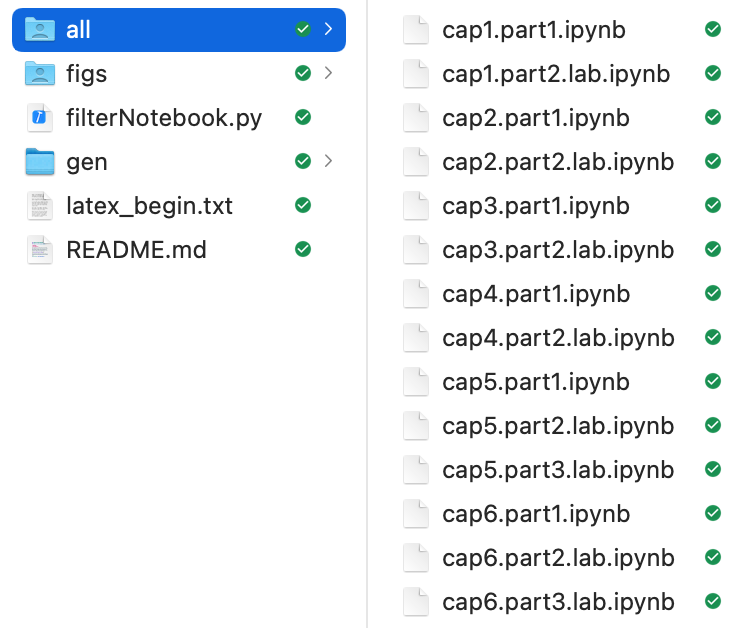
\includegraphics[width=.37\textwidth]{cap13_fig01}
\raisebox{15.3\height}{(b)}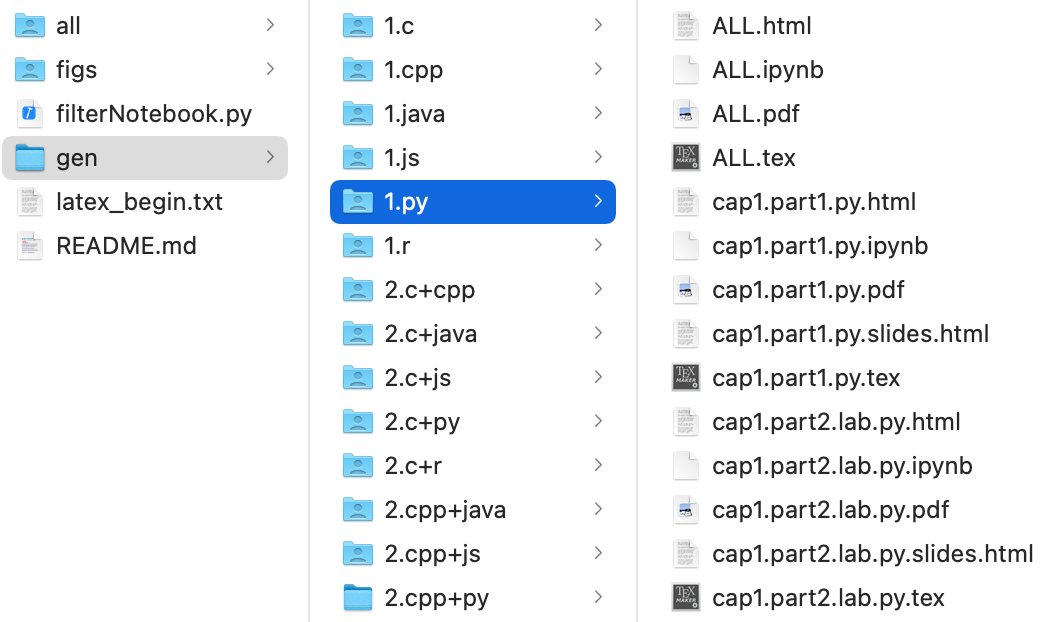
\includegraphics[width=.53\textwidth]{cap13_fig03} 
\caption{(a) estrutura de arquivos e pastas; (b) recorte da estrutura de arquivos e pastas gerados automaticamente, detalhando a pasta \texttt{1.py} para Python. Fonte: \citeonline{2021:Zampirolli.Teubl.ea}.}
\label{fig:pastaAll}
\end{figure}

  
Em cada arquivo \verb|ipynb| da pasta ``all'' da Figura \ref{fig:pastaAll}, a primeira linha de cada célula, seja de texto ou código, pode conter a(s) linguagem(ns) de programação escolhida(s) para o conteúdo daquela célula. Isso segue a sintaxe \verb|#[tipo1]#[tipo2]#...#[tipon]#|, em que \verb|tipoi| é a extensão do arquivo do código na linguagem escolhida.

O filtro \verb|filterNotebook.py|, disponível em \href{https://github.com/fzampirolli/filterNotebook}{github.com/fzampirolli/filterNotebook}, permite filtrar \textit{notebooks} com base na linguagem de programação e convertê-los para os formatos HTML, LaTeX e PDF. Essa ferramenta suporta várias linguagens de programação, e o número de combinações possíveis depende do número de linguagens definidas.


\subsubsection{Experimentos}

O método foi validado em 5 turmas remotas, totalizando 223 estudantes, com uma taxa média de aprovação de 90\%. Ele se mostrou facilmente adaptável e oferece flexibilidade aos estudantes, possibilitando uma abordagem mais personalizada no processo de aprendizagem de programação.

Os estudantes da disciplina CS1 foram divididos em dois grupos. O Grupo 1 teve aulas síncronas (teóricas e práticas) e os estudantes foram obrigados a gravar vídeos explicativos para as atividades. O Grupo 2 teve aulas assíncronas e os estudantes não foram obrigados a gravar vídeos explicativos. Os resultados do questionário aplicado aos estudantes mostraram que o Grupo 1 teve uma avaliação mais positiva da disciplina do que o Grupo 2. Em particular, os estudantes do Grupo 1 ficaram mais satisfeitos com as aulas síncronas, com o material didático e com as avaliações. A análise estatística também mostrou que o método aplicado ao Grupo 1 foi estatisticamente melhor do que o método aplicado ao Grupo 2.
%
Os estudantes dos dois grupos concordaram que a disciplina foi importante para aprender sobre programação e o conhecimento de várias linguagens de programação é útil para a carreira profissional.

Os resultados deste estudo sugerem que as aulas síncronas podem ser uma forma eficaz de ensinar programação. No entanto, é importante que as aulas síncronas sejam bem planejadas e os estudantes sejam motivados a participar.

%%%%%%%%%%%%%%%%%%%%%%%%%%%%%%%%%%%%%%%%%%%%%%%%%%%%%%%%%%%%%%%%%%%%%%%%%
\subsection{Artigo aplicando a integração MCTest+Moodle+VPL em CS1}
%%%%%%%%%%%%%%%%%%%%%%%%%%%%%%%%%%%%%%%%%%%%%%%%%%%%%%%%%%%%%%%%%%%%%%%%%

O artigo de \citeonline{2021:Zampirolli.Josko.ea}, publicado na revista \textit{Computer Applications in Engineering Education} e resumido nesta seção, descreve um experimento significativo envolvendo a implementação do método apresentado na Seção \ref{sec:MCTest-5web} -- \nameref{sec:MCTest-5web} \cite{2020:Zampirolli.Pisani.ea}. Esse estudo complementa um artigo anterior publicado na mesma revista, resumido na Seção \ref{sec:experMCTest-4revista} -- \nameref{sec:experMCTest-4revista} \cite{2018:Zampirolli.Goya.ea}.

Nesse novo estudo, a integração MCTest+Moodle+VPL foi incorporada como parte do processo de ensino e avaliação na disciplina CS1. Inicialmente, tentou-se publicar tanto o método quanto o experimento em um único artigo nesta revista. No entanto, os revisores consideraram o conteúdo muito denso, o que levou à separação em dois artigos distintos: \citeonline{2020:Zampirolli.Pisani.ea} e \citeonline{2021:Zampirolli.Josko.ea}.


\subsubsection{Método}

A principal característica da abordagem consiste na implementação da avaliação automatizada (AA) em uma disciplina CS1 com várias turmas. Esse método engloba a formulação de questões individuais para cada estudante e a disponibilização de avaliação e \textit{feedback} automáticos.

Para a realização da avaliação unificada, foram empregadas questões paramétricas e respostas (nos casos de QMs) através do MCTest. Essa estratégia possibilitou a combinação de distintos tipos de questões para gerar um exame personalizado para cada estudante. Já para as QTs, foi utilizada a integração MCTest+Moodle+VPL, na qual os estudantes tiveram que submeter EPs em atividades VPL do Moodle.

%Como resultado, foram gerados arquivos PDF individuais para cada estudante. Essa abordagem permitiu uma análise precisa do desempenho de cada estudante, com AA e \textit{feedback} imediato, tornando o processo de avaliação mais eficiente e efetivo.

Importante destacar que todo o processo avaliativo utilizado neste artigo foi previamente detalhado e exemplificado em capítulos anteriores deste livro. Além disso, é possível criar várias turmas pelo coordenador de disciplina, conforme detalhado na Seção \ref{sec:variasTurmasCSV} -- \nameref{sec:variasTurmasCSV}. Da mesma forma, é explicado no Capítulo \ref{ch:exames} -- \nameref{ch:exames} como enviar um exame também para várias turmas.

\subsubsection{Experimentos}

A principal característica do experimento realizado é a capacidade de aplicar AA e exames unificados parametrizados em diferentes linguagens de programação, utilizando as ferramentas de código aberto MCTest e Moodle (com o \textit{plugin} VPL). No primeiro trimestre de 2019, 19 das 44 turmas (presenciais) adotaram a abordagem, alcançando uma taxa de aprovação mais alta (67,5\%) em comparação com as turmas que não utilizaram a solução de AA (59,1\%), mantendo uma dispersão padrão semelhante. Resultados preliminares também indicaram uma forte correlação linear entre a taxa de aprovação e a média das notas nas AA. Nas turmas de aprendizagem mista (\textit{blended learning}), duas turmas utilizaram o método nos exames unificados, com uma taxa de aprovação de 70,4\%. Esses resultados corroboram estudos anteriores, indicando que a avaliação contínua combinada com \textit{feedback} imediato pode contribuir para o processo de aprendizagem dos estudantes. 

%%%%%%%%%%%%%%%%%%%%%%%%%%%%%%%%%%%%%%%%%%%%%%%%%%%%%%%%%%%%%%%%%%%%%%%%%
\subsection{Artigo explorando a integração de jogos no ensino de CS0}
%%%%%%%%%%%%%%%%%%%%%%%%%%%%%%%%%%%%%%%%%%%%%%%%%%%%%%%%%%%%%%%%%%%%%%%%%

O artigo de \citeonline{2023:Josko.Zampirolli} discute uma intervenção pedagógica que emprega elementos de gamificação para a introdução de conceitos de lógica de programação em estudantes. No estudo, os autores realizaram um estudo de caso envolvendo 48 estudantes matriculados no curso introdutório de programação (CS0) intitulado Bases Computacionais da Ciência, parte do programa de Bacharelado em Ciência e Tecnologia da UFABC. Importante ressaltar que o curso foi ministrado \textit{online} devido à pandemia.

\subsubsection{Método}

A intervenção pedagógica consistiu em construir gradualmente um jogo simples utilizando a biblioteca Pygame (\href{https://www.pygame.org/news}{pygame.org}) do Python no Google Colab (\href{https://colab.google/}{colab.google}). Conceitos como instruções sequenciais, bibliotecas, estruturas de decisão e de repetição, além de simulações, foram introduzidos à medida que novas funcionalidades eram incluídas no jogo. Além disso, foram utilizadas avaliações automáticas e \textit{feedback} para os estudantes, conforme relatado em outro artigo descrito na Seção \ref{sec:mctest_cs0_2021} -- \nameref{sec:mctest_cs0_2021}.

\subsubsection{Experimentos}

Os autores aplicaram um questionário para capturar as perspectivas dos estudantes sobre a abordagem. As análises sugeriram que os elementos de gamificação melhoraram a motivação em relação aos tópicos do curso. Adicionalmente, a taxa de reprovação do grupo estudado foi menor do que a média de outras turmas no período da pandemia.

Assim, a intervenção recebeu \textit{feedback} positivo dos estudantes. Entretanto, os autores afirmam que estudos controlados com maiores amostras são necessários para avaliar plenamente a efetividade da abordagem. 


%%%%%%%%%%%%%%%%%%%%%%%%%%%%%%%%%%%%%%%%%%%%%%%%%%%%%%%%%%%%%%%%%%%%%%%%%
\section{Aplicação do MCTest-5 com Moodle+VPL no Ensino de PDI}\label{sec:mctest+moodle+vpl+pdi}
%%%%%%%%%%%%%%%%%%%%%%%%%%%%%%%%%%%%%%%%%%%%%%%%%%%%%%%%%%%%%%%%%%%%%%%%%

Ao contrário dos artigos apresentados na Seção \ref{sec:mctest+moodle+vpl}, que descrevem experimentos em cursos introdutórios de lógica de programação (CS0 e CS1), esta seção relata a aplicação dessa integração no curso de Processamento Digital de Imagens (PDI).

O trabalho ``\texttt{A Practical Digital Image Processing Course with \texttt{morph.py}}'' de \citeonline{2024:Zampirolli.Josko-PDI} foi publicado no Simpósio Brasileiro de Ensino de Computação e \textbf{recebeu o primeiro lugar na categoria de Recursos e Ambientes Educacionais} entre os trabalhos apresentados no evento.

Isso marca o encerramento de um ciclo virtuoso iniciado em 2012, com a primeira publicação de \citeonline{2013:Zampirolli.Quilici-Gonzalez.ea} relacionada ao PDI na primeira versão do MCTest, ainda em Matlab, introduzido no primeiro capítulo deste livro, na Seção \ref{sec:historico} -- \nameref{sec:historico}.

O ensino de PDI é desafiador devido à sua complexidade matemática e algorítmica. Este artigo apresenta um curso prático que utiliza a biblioteca Python \texttt{morph.py} para apoiar o ensino. O curso interativo emprega exemplos ilustrativos e exercícios práticos para facilitar a compreensão de conceitos e operadores fundamentais de PDI, desde noções básicas até tópicos avançados. Um estudo de caso exploratório com um grupo de 15 participantes confirmou a eficácia do método de ensino baseado na biblioteca \texttt{morph.py}, abordando as dificuldades de ensinar PDI a iniciantes.


\subsection{Método}

Nesta seção, é resumido o método apresentado no artigo, contextualizando o curso de PDI e detalhando a intervenção pedagógica, com ênfase na utilização da biblioteca \verb|morph.py| como um fator motivacional. Por fim, foi discutido os ambientes de desenvolvimento.

\subsubsection{Contexto} \label{sec:cont}

O curso de PDI é uma disciplina eletiva oferecida a estudantes de diversos programas na universidade, como o Bacharelado em Ciência da Computação e vários cursos de Engenharia. Com duração de 12 semanas e quatro horas de aula por semana, o curso é ministrado por meio de aulas laboratoriais síncronas, onde os professores apresentam Colabs contendo conceitos, exemplos e exercícios no Sistema de Gerenciamento de Aprendizado Moodle. Em 2023, o curso foi oferecido para 25 estudantes de fevereiro a maio, incluindo aulas gravadas produzidas durante a pandemia de Covid-19.

\subsubsection{Intervenção Pedagógica} \label{sec:pi}

O curso aborda uma ampla gama de tópicos em PDI, com as primeiras seis semanas dedicadas a equipar os estudantes com habilidades essenciais para desenvolver operadores de PDI, como limiares, histogramas, convolução, erosão, dilatação, filtros, \textit{watershed}, rotulagem e transformações de distância, seguindo o livro-texto de Gonzalez e Woods \cite{gonzalez2009processamento}. Na sétima semana, os estudantes fazem o Exame 1, enquanto as semanas subsequentes (oito a dez) focam na aplicação desses operadores de PDI para resolver problemas reais de visão computacional. Em suma, a primeira parte do curso visa fornecer aos estudantes as habilidades necessárias para desenvolver operadores de PDI, enquanto a segunda parte constrói sobre essa base, aplicando esses operadores para resolver vários problemas de visão computacional. A semana onze é reservada para revisão, e o curso é concluído com um exame final na semana doze.

A avaliação do curso consiste em quatro tarefas individualizadas e parametrizadas (15\% da nota final), relacionadas ao último tópico abordado em sala de aula. Essas tarefas são fornecidas aos emails dos estudantes antes de cada aula e são avaliadas automaticamente utilizando a integração do MCTest, Moodle e VPL \cite{2020:Zampirolli.Pisani.ea,2021:Zampirolli.Sato.ea}. Além dessas tarefas, o Exame 1 (30\% da nota final) consiste em exercícios semelhantes. Para o projeto individual final (15\% da nota final), os estudantes devem desenvolver um Colab para resolver um problema de PDI. O exame final (40\% da nota final) segue uma estrutura similar ao projeto. Tanto o primeiro quanto o último exame devem ser concluídos dentro do período de duas horas de aula.

\subsubsection{Ambientes de Desenvolvimento}\label{sec:development}

A Figura~\ref{fig:cap13_DIP01} fornece uma visão geral da intervenção pedagógica empregada no curso de PDI, utilizando a biblioteca \verb|morph.py|, que oferece 71 métodos, incluindo operações (como mínimo, máximo e negação) e operadores (como erosões e dilatações). Embora o curso ia870p3\footnote{Disponível em \url{http://github.com/robertoalotufo/ia870p3}.} \cite{ia898p3} tenha abordado alguns algoritmos da caixa de ferramentas \verb|mmorph|~\cite{dougherty2003hands}, nem esse curso nem o curso apresentado no artigo cobriram toda a gama de funcionalidades oferecidas pela caixa de ferramentas.

O material do curso consistiu em seis \textit{notebooks} conceituais durante as seis primeiras semanas e oito documentos focados em operadores morfológicos. Esses recursos foram utilizados até o Exame 1, marcando um marco significativo na progressão do curso. Após o Exame 1, o curso incorporou um conjunto de 27 demonstrações de \textit{notebooks} que combinavam teoria com prática.

\begin{figure}[ht]
\centering
   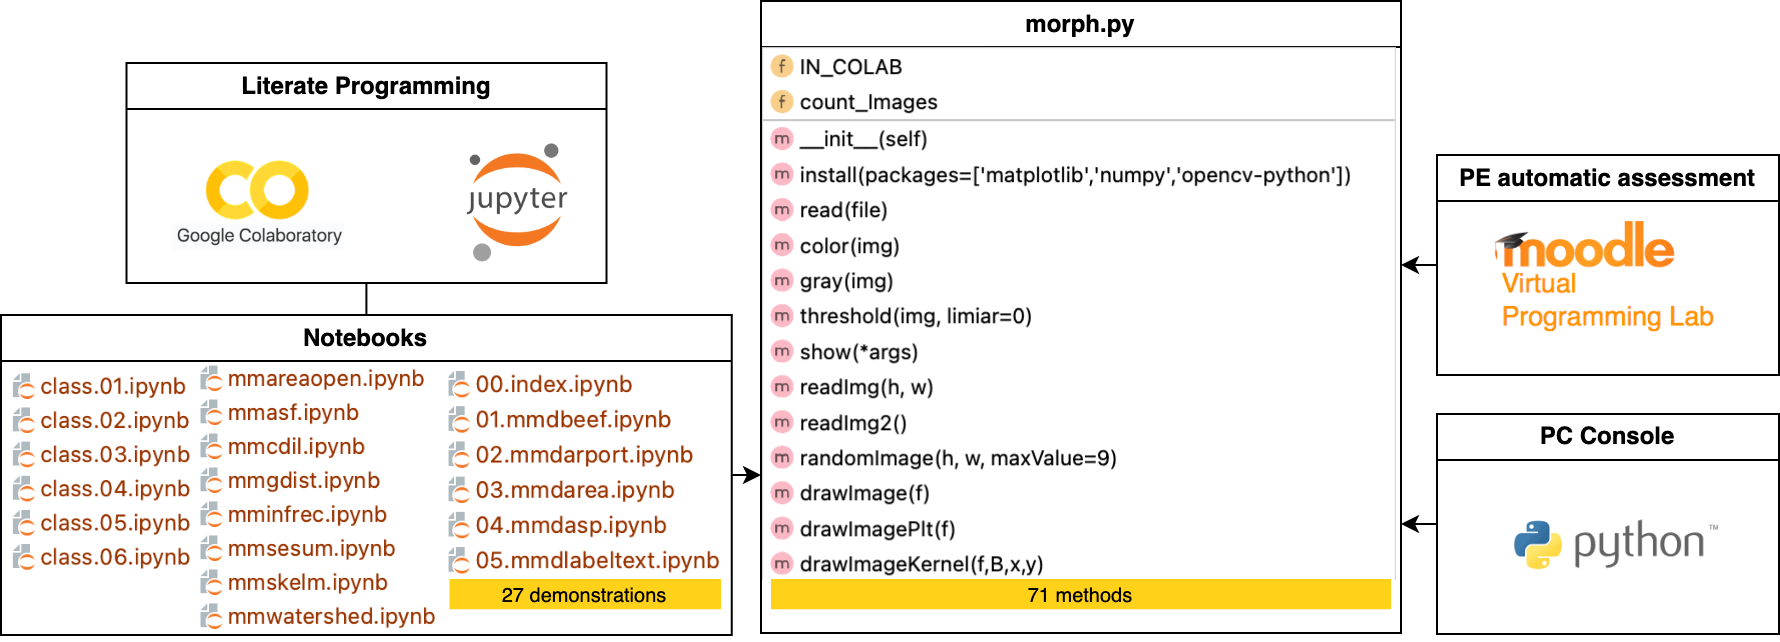
\includegraphics[width=0.99\textwidth]{cap13_DIP01.png}
\caption{Visão geral da intervenção pedagógica empregada no curso de PDI. Fonte: \cite{2024:Zampirolli.Josko-PDI}.}
\label{fig:cap13_DIP01}
\end{figure}

Agora, o sistema de VPL fornece uma abordagem automatizada para avaliar as soluções dos estudantes. Por meio da biblioteca \verb|morph.py|, é possível verificar diretamente as soluções dos estudantes e compará-las com as respostas corretas, agilizando o processo de avaliação. Além disso, a combinação de \textit{notebooks} conceituais com \textit{notebooks} de demonstração permite aos estudantes uma compreensão completa dos conceitos, seguida pela aplicação prática desses conceitos em exemplos específicos. Essa abordagem integrada ajuda a fortalecer a compreensão dos estudantes e a solidificar suas habilidades práticas em PDI.

\subsection{Experimentos}

Os autores realizaram uma pesquisa voluntária para coletar dados dos estudantes em nosso curso de PDI. A pesquisa foi administrada após o exame final e incluiu 5 perguntas baseadas em Likert para obter \textit{feedback} sobre o conteúdo e as estratégias do curso.

Dos estudantes que concluíram o curso, foram 15 respostas (aproximadamente 60\%). Os autores analisaram essas respostas e descobriram que duas perguntas se assemelham a uma distribuição normal. Portanto, foi utilizado um método paramétrico (\textit{teste t}) para essas duas perguntas e um método não paramétrico equivalente (\textit{Wilcoxon Signed-Rank}) para as restantes. Além disso, foi aplicado o Alpha de Cronbach para avaliar a consistência interna dos dados Likert, obtendo um valor de 0,90. Finalmente, foi testada a hipótese de que a biblioteca \texttt{morph.py} teve um efeito neutro na aprendizagem dos estudantes.

Os resultados mostram diferenças significativas entre todas as perguntas e a hipótese nula. Por exemplo, a percepção positiva dos estudantes sobre a biblioteca indica que ela facilitou a exploração dos diferentes algoritmos pré-implementados sem a necessidade de implementá-los do zero. Como resultado, eles puderam se concentrar mais em entender os conceitos subjacentes e as técnicas por trás dos algoritmos, reduzindo a curva de aprendizado inicial. Finalmente, dos 25 estudantes que concluíram o curso, apenas 4 não obtiveram aprovação, resultando em uma taxa de aprovação de 84\%.

Desafios à validade incluem a natureza eletiva do curso de PDI na universidade, o que pode afetar a representatividade dos resultados. Além disso, a realização de experimentos envolvendo grupos de teste e controle requer aprovação do comitê de ética e apresenta desafios logísticos. Assim, este estudo abre caminho para pesquisas futuras explorarem novas formas de experimentação.


\section{Considerações finais}

Neste capítulo, foram apresentados vários artigos que relatam experiências importantes com a integração do MCTest com o Moodle e o \textit{plugin} VPL. Essas integrações permitiram a avaliação automatizada de EPs em diversas disciplinas, com destaque para:

\begin{itemize}
    \item Criação de QTs paramétricas e de QMs corrigidas manualmente e automaticamente;
    \item Exportação de questões do MCTest para o banco de questões do Moodle, superando limitações;
    \item Geração de listas unificadas de EPs paramétricos com casos de teste automatizados;
    \item Disponibilização de material didático e avaliativo em várias linguagens de programação;
    \item Uso de avaliação contínua e \textit{feedback} imediato, resultando em maior taxa de aprovação.
\end{itemize}

Os artigos apresentam a evolução e aprimoramentos dessas integrações ao longo do tempo. Além disso, foi observado que as turmas que utilizaram os métodos propostos tiveram um desempenho melhor. No entanto, é difícil afirmar que essa foi a única razão para o melhor desempenho.

Portanto, é possível concluir que as abordagens propostas neste capítulo se mostraram eficazes e práticas, especialmente no contexto de ensino remoto durante a pandemia COVID-19. Essas integrações abrem novas possibilidades para oferecer avaliações personalizadas, automatizadas e flexíveis em diversas disciplinas, como as de programação.
